\documentclass[11pt,preprint, authoryear]{elsarticle}

\usepackage{lmodern}
%%%% My spacing
\usepackage{setspace}
\setstretch{1.2}
\DeclareMathSizes{12}{14}{10}{10}

% Wrap around which gives all figures included the [H] command, or places it "here". This can be tedious to code in Rmarkdown.
\usepackage{float}
\let\origfigure\figure
\let\endorigfigure\endfigure
\renewenvironment{figure}[1][2] {
    \expandafter\origfigure\expandafter[H]
} {
    \endorigfigure
}

\let\origtable\table
\let\endorigtable\endtable
\renewenvironment{table}[1][2] {
    \expandafter\origtable\expandafter[H]
} {
    \endorigtable
}


\usepackage{ifxetex,ifluatex}
\usepackage{fixltx2e} % provides \textsubscript
\ifnum 0\ifxetex 1\fi\ifluatex 1\fi=0 % if pdftex
  \usepackage[T1]{fontenc}
  \usepackage[utf8]{inputenc}
\else % if luatex or xelatex
  \ifxetex
    \usepackage{mathspec}
    \usepackage{xltxtra,xunicode}
  \else
    \usepackage{fontspec}
  \fi
  \defaultfontfeatures{Mapping=tex-text,Scale=MatchLowercase}
  \newcommand{\euro}{€}
\fi

\usepackage{amssymb, amsmath, amsthm, amsfonts}

\def\bibsection{\section*{References}} %%% Make "References" appear before bibliography


\usepackage[round]{natbib}

\usepackage{longtable}
\usepackage[margin=2.3cm,bottom=2cm,top=2.5cm, includefoot]{geometry}
\usepackage{fancyhdr}
\usepackage[bottom, hang, flushmargin]{footmisc}
\usepackage{graphicx}
\numberwithin{equation}{section}
\numberwithin{figure}{section}
\numberwithin{table}{section}
\setlength{\parindent}{0cm}
\setlength{\parskip}{1.3ex plus 0.5ex minus 0.3ex}
\usepackage{textcomp}
\renewcommand{\headrulewidth}{0.2pt}
\renewcommand{\footrulewidth}{0.3pt}

\usepackage{array}
\newcolumntype{x}[1]{>{\centering\arraybackslash\hspace{0pt}}p{#1}}

%%%%  Remove the "preprint submitted to" part. Don't worry about this either, it just looks better without it:
\makeatletter
\def\ps@pprintTitle{%
  \let\@oddhead\@empty
  \let\@evenhead\@empty
  \let\@oddfoot\@empty
  \let\@evenfoot\@oddfoot
}
\makeatother

 \def\tightlist{} % This allows for subbullets!

\usepackage{hyperref}
\hypersetup{breaklinks=true,
            bookmarks=true,
            colorlinks=true,
            citecolor=blue,
            urlcolor=blue,
            linkcolor=blue,
            pdfborder={0 0 0}}


% The following packages allow huxtable to work:
\usepackage{siunitx}
\usepackage{multirow}
\usepackage{hhline}
\usepackage{calc}
\usepackage{tabularx}
\usepackage{booktabs}
\usepackage{caption}


\newenvironment{columns}[1][]{}{}

\newenvironment{column}[1]{\begin{minipage}{#1}\ignorespaces}{%
\end{minipage}
\ifhmode\unskip\fi
\aftergroup\useignorespacesandallpars}

\def\useignorespacesandallpars#1\ignorespaces\fi{%
#1\fi\ignorespacesandallpars}

\makeatletter
\def\ignorespacesandallpars{%
  \@ifnextchar\par
    {\expandafter\ignorespacesandallpars\@gobble}%
    {}%
}
\makeatother

\newenvironment{CSLReferences}[2]{%
}

\urlstyle{same}  % don't use monospace font for urls
\setlength{\parindent}{0pt}
\setlength{\parskip}{6pt plus 2pt minus 1pt}
\setlength{\emergencystretch}{3em}  % prevent overfull lines
\setcounter{secnumdepth}{5}

%%% Use protect on footnotes to avoid problems with footnotes in titles
\let\rmarkdownfootnote\footnote%
\def\footnote{\protect\rmarkdownfootnote}
\IfFileExists{upquote.sty}{\usepackage{upquote}}{}

%%% Include extra packages specified by user
\usepackage{booktabs}
\usepackage{longtable}
\usepackage{array}
\usepackage{multirow}
\usepackage{wrapfig}
\usepackage{float}
\usepackage{colortbl}
\usepackage{pdflscape}
\usepackage{tabu}
\usepackage{threeparttable}
\usepackage{threeparttablex}
\usepackage[normalem]{ulem}
\usepackage{makecell}
\usepackage{xcolor}

%%% Hard setting column skips for reports - this ensures greater consistency and control over the length settings in the document.
%% page layout
%% paragraphs
\setlength{\baselineskip}{12pt plus 0pt minus 0pt}
\setlength{\parskip}{12pt plus 0pt minus 0pt}
\setlength{\parindent}{0pt plus 0pt minus 0pt}
%% floats
\setlength{\floatsep}{12pt plus 0 pt minus 0pt}
\setlength{\textfloatsep}{20pt plus 0pt minus 0pt}
\setlength{\intextsep}{14pt plus 0pt minus 0pt}
\setlength{\dbltextfloatsep}{20pt plus 0pt minus 0pt}
\setlength{\dblfloatsep}{14pt plus 0pt minus 0pt}
%% maths
\setlength{\abovedisplayskip}{12pt plus 0pt minus 0pt}
\setlength{\belowdisplayskip}{12pt plus 0pt minus 0pt}
%% lists
\setlength{\topsep}{10pt plus 0pt minus 0pt}
\setlength{\partopsep}{3pt plus 0pt minus 0pt}
\setlength{\itemsep}{5pt plus 0pt minus 0pt}
\setlength{\labelsep}{8mm plus 0mm minus 0mm}
\setlength{\parsep}{\the\parskip}
\setlength{\listparindent}{\the\parindent}
%% verbatim
\setlength{\fboxsep}{5pt plus 0pt minus 0pt}



\begin{document}



\begin{frontmatter}  %

\title{Navigating the Stock Market: A Guide to Smart Investing}

% Set to FALSE if wanting to remove title (for submission)




\author[Add1]{Gabriel Rambanapasi}
\ead{rambanapasi44@gmail.com}





\address[Add1]{Stellenbosch University, Stellenbosch, South Africa}

\cortext[cor]{Corresponding author: Gabriel Rambanapasi}

\begin{abstract}
\small{
This paper investigates dividends return predictive signals, focusing on
Dividend Yield (DY) and Dividend Growth (DG) signals, w
}
\end{abstract}

\vspace{1cm}


\begin{keyword}
\footnotesize{
K-Means\sep Clustering \sep Price Momentun \sep Volatility
\sep Diversification \\
\vspace{0.3cm}
}
\end{keyword}



\vspace{0.5cm}

\end{frontmatter}

\setcounter{footnote}{0}



%________________________
% Header and Footers
%%%%%%%%%%%%%%%%%%%%%%%%%%%%%%%%%
\pagestyle{fancy}
\chead{}
\rhead{}
\lfoot{}
\rfoot{\footnotesize Page \thepage}
\lhead{}
%\rfoot{\footnotesize Page \thepage } % "e.g. Page 2"
\cfoot{}

%\setlength\headheight{30pt}
%%%%%%%%%%%%%%%%%%%%%%%%%%%%%%%%%
%________________________

\headsep 35pt % So that header does not go over title




\hypertarget{introduction}{%
\section{Introduction}\label{introduction}}

Consider the prevailing market consensus that anticipates a specific
direction for market conditions. For instance, in the current interest
rate environment, the majority of practitioners believe that in 2024,
the Federal Reserve will initiate interest rate cuts. This could trigger
a chain reaction in valuations across capital markets, affecting sectors
and industries disproportionately. For investors, this underscores the
importance of carefully scrutinizing different parts of the stock market
to pinpoint companies that can enhance the risk/return profile of a
portfolio. We set out to employ a combination of K-Means clustering and
technical factors. Essentially, we reduce the dimensions of our sample
data, to create ``cluster portfolios'' making it less challenging to
uncover latent relationships in asset performance and group
characteristics.

Our initial assessment involves the utilization of a simple look-back
period to observe performance and risk over 3, 6, and 12 months. This
analysis reveals that, on average, cluster portfolios exhibit strong
performance over short investment horizons. However, they also display
significant risk levels when compared to a market index. To further
evaluate the robustness of the portfolios formed through our factor
filter, we conduct a rolling backtest. The findings suggest that,
despite the elevated levels of risk attributed to the low number of
stocks in each portfolio, risk-adjusted performance, as measured by the
Sharpe Ratio (SR), returns strong positive performance over short time
horizons. It is noteworthy that this strategy demonstrates effectiveness
over shorter investment horizons. However, as the investment horizon
extends, the superior risk adjsuted return flatuates and diminishes.

This integrated approach of clustering and factor analysis provides a
valuable toolkit for portfolio managers seeking to identify potential
out performers admidst anticipated market shifts. The focus on reducing
the complexity of the data allows for a more nuanced understanding of
asset performance, with the potential for enhanced risk-adjusted returns
in the short term. Nevertheless, the strategy's limitations in the
context of underscore the importance of continual refinement and
adaptation to evolving market conditions.

The next section \ref{lit} offers a brief discription of the various
unsupervised machine learning algorithms. Section \ref{meth} details the
methodology and data used along with its preparation procedure to be
utilized by the K means clustering algorithm. Section \ref{Results}
discusses the results and sectiom \ref{con} offers the conclusion.

\hypertarget{clustering-and-appliactions-to-asset-management}{%
\section{\texorpdfstring{Clustering and Appliactions to Asset Management
\label{lit}}{Clustering and Appliactions to Asset Management }}\label{clustering-and-appliactions-to-asset-management}}

Unsupervised machine learning is a type of machine learning that
searches for patterns in datasets with no pre-existing labels and a
minimum of human intervention. One way in which unsupervised learning
can be applied in data science and other quantitive disciplines is
through clustering algorithms. Clustering is the process of grouping
objects based on similar characteristics. The algorithms designed to
cluster, achieve this function by connecting observation through
distances, density of data points, graphs, or various statistical
distributions. For a cluster to have meaning an algorithm has to
maximize intra-cluster similarity and minimize inter-cluster similarity,
such that each cluster contains information that's as dissimilar to
other
clusters(\protect\hyperlink{ref-kassambara2017practical}{Kassambara,
2017}). There exists various forms of cluster algorithms, each that
addresses a broader task of analysis. The algorithms can be divided into
two main types being partitioning clustering and hierarchical
clustering. The major difference between the divisions of clustering is
the partition clustering aims to specify a predetermined number of
clusters whilst does not
(\protect\hyperlink{ref-kassambara2017practical}{Kassambara, 2017}).
Within partition clustering, for data with a small set of variables,
K-means clustering and partitioning around medoids (PAM) are the most
frequently used due to their fast compuation and simplicity. With
K-means, each cluster is represented by the center or means of the data
points belonging to the entire dataset. This makes the algorithm
sensitive to outliers. However with PAM, each cluster is represented by
one of the objects in the cluster. The other partition clustering
algorithm used for datasets with a large number of variables is
Clustering Large Applications (CLARA).

In asset management, key to funds generating superior risk adjusted
returns is efficient portfolio diversification, thus presenting a great
application for partition clustering. Stocks would be separated into
groups through a clustering algorithm to maximize similarity within
groups and minimizes similarity between groups. Thus allowing managers
to select handpick stock to construct a diversified portfolio. Marvin
(\protect\hyperlink{ref-marvin2015creating}{2015}) use fundamental
ratios (turnover and profitability ratios) weighted equally and K-means
clustering to group US technology stocks listed on the NASDAQ and NYSE.
A diversified portfolio is then constructed based on within cluster
stock performance i.e.~stock selected are those that possess the highest
Sharpe ratio. Results over a period of 15 years that included the dot
com bubble and the global financial crises showed that cluster
portfolios exhibited more volatility than the benchmark (S\&P 500),
however returns to investors were above the benchmark at multiples
ranging from 3.5 to 5.7 times when earnings are reinvested into the
cluster portfolios. Bin (\protect\hyperlink{ref-bin2020k}{2020}) uses a
similar approach to Marvin
(\protect\hyperlink{ref-marvin2015creating}{2015}), however employing a
combination of market ratios and fundamental ratios (price to earnings
ratio, return on assets ratio and asset turnover ratio ). From this
study, compared to the S\&P 500, portfolios constructed using market
ratios under performed those that used fundamental ratios. \newpage

\hypertarget{data-and-methodology}{%
\section{\texorpdfstring{Data and Methodology
\label{meth}}{Data and Methodology }}\label{data-and-methodology}}

This section describes how we obtain the data set used in the study,
details the clustering process and validating metrics employed, to
obtain the results in \ref{Results}. For the methodology results, see
Appendix \ref{app1} and \ref{app2}.

\hypertarget{obtaining-and-prepariing-the-dataset}{%
\subsection{Obtaining and prepariing the
dataset}\label{obtaining-and-prepariing-the-dataset}}

The data employed in this paper is based on the constituent list of the
Johannesburg All Share Index (ALSI) from January 1, 2014 to January 29
2024. The historical price and volume data is retrieved from Yahoo
Finance. From historical price data obtained from Yahoo Finance, we
filter stock that have trading volume that exceed 1 000 000 shares
traded per year and exclude stock that have less than 90 percent of
observations in the historical price dataset.

To avoid large oscillations in the data, we transformed the price series
to include end of month data points thus returns calculations are based
on from the monthly data. Monthly historical prices are transformed
using simple returns and we assume that embedded in the price action are
cooperate events such as stock splits or consolidations of the shares.
Therefore there is no need to make additional transformations on the
return series to reflect corporate actions.

The measures of similarity used in this study are volatility and price
momentum. To cluster stock based on the two measures, we apply a
percentile ranking criterion on stock scores during a time period. For
price momentum, describes the causality between relatively strong
performance and high future return and vice-versa. Ranking highly
implies that strong performers and thus higher returns than weak
performers. This study defines cross sectional momentum as the trailing
12 month cumulative return Jegadeesh \& Titman
(\protect\hyperlink{ref-jegadeesh1993returns}{1993}), a modication to
capture some longer term effects in the return series. For volatility,
using a 12 month lock back period compute the standard deviation. The
results of the ranking are shown in Table \ref{tab1}

\hypertarget{stocks-clustering}{%
\subsection{Stocks clustering}\label{stocks-clustering}}

\hypertarget{lloyds-algorithm}{%
\subsubsection{Lloyd's algorithm}\label{lloyds-algorithm}}

We employ the K-means that partitions \(n\) observations into \(k\)
clusters. The goal is to minimize the within cluster sum of squares or
analytically,
\(\underset{s}{\arg \min } \sum_{i=1}^k \sum_{x \in S_i}\left\|x-\mu_i\right\|^2\)
where \(x\) are the observations, \(S=S_1, S_2, \ldots, S_k\) are the
sets of observations, and \(\mu_i\) is the mean of the points in
\(S_i\). To arrive at the optimum number of clusters, we utilize the
most popular algorithm called the Lloyd's algorithm that is closely
followed by Marvin (\protect\hyperlink{ref-marvin2015creating}{2015}),
Bin (\protect\hyperlink{ref-bin2020k}{2020}) \& Xu, Xu \& Wunsch
(\protect\hyperlink{ref-xu2010clustering}{2010}).

Analytically, given a set of points
\(\left\{x_1, \cdots x_n\right\}\left(x_i \in \mathbb{R}^m\right)\),
Initialize the K clusters with \(\left\{C_1, \cdots C_K\right\}\) with
centers.
\(\left\{m_1, m_2, \cdots m_K\right\}\left(m_i \in \mathbb{R}^m\right)\).
The centers are picked using the silhouette method discussed in
\ref{sil} For all points \(x_i(i \in\{1, \cdots n\})\), find the center
that closest based on a euclidean distance \(d\). Following this, assign
\(x_i\) to the cluster corresponding to the closest centre. Then
\(x_i \in C_j\) if
\(d\left(x_i, m_j\right) \leq d\left(x_i, m_l\right) \quad(\forall l \in\{1, \cdots K\})(j \neq l)(\forall i \in\{1, \cdots n\})\).
Recalculate the center for each cluster \(C_l(l \in\{1, \cdots K\})\).
The new cluster centers are the mean of the points in the same cluster.

\(m_l=\frac{1}{\left|C_l\right|} \sum_{x_p \in C_l} x_p \quad(\forall l \in\{1, \cdots K\})\).

Repeat processes two and three until no cluster has any change in point
assignment.

\hypertarget{silhoutte-index}{%
\subsection{\texorpdfstring{Silhoutte index
\label{sil}}{Silhoutte index }}\label{silhoutte-index}}

To evaluate the goodness of fit of partitioning using K means clustering
the silhoutte index is used
(\protect\hyperlink{ref-rousseeuw1987silhouettes}{Rousseeuw, 1987}).
Given \(n\) data points \(\left\{x_1, \cdots x_n\right\}\), a
partitioning result of \(K\) cluster \(\left\{C_1, \cdots C_K\right\}\)
and distance metric \(d\), for each \(x_i\) in cluster \(C_l\), define

\(a\left(x_i\right)=\frac{1}{\left|C_l\right|-1} \sum_{\forall x_j \in C_l, i \neq j} d\left(x_i, x_j\right)\)

\(a(x_i)\) is the mean dissimilarity between \(x_i\) to all other points
within the same cluster.For each point \(x_i\) in cluster \(C_l\),
define

\(b\left(x_i\right)=\min _{\forall p \in\{1, \cdots K\}, p \neq l} \frac{1}{\left|C_p\right|} \sum d\left(x_i, x_j\right.)\)

\(b(x_i)\) is the minimum dissimilarity between \(x_i\) and all points
in some \(C_p\) which does not contain \(x_i\). For each point \(x_i\)
in cluster \(C_l\), their silhouette index is defined as

\(s\left(x_i\right)= \begin{cases}1-\frac{a\left(x_i\right)}{b\left(x_i\right)} & \text { if } a\left(x_i\right)<b\left(x_i\right) \\ 0 & \text { if } a\left(x_i\right)=b\left(x_i\right) \\ \frac{b\left(x_i\right)}{a\left(x_i\right)}-1 & \text { if } a\left(x_i\right)>b\left(x_i\right)\end{cases}\)

where \(s(x_i)\) ranges between \([-1, 1]\). For \(s(x_i)\) that
approaches 1, it means that \(a(x_i)\) needs to be significantly smaller
than \(b(x_i)\), implying that within-cluster mean dissimilarity is much
less than the smallest between-cluster mean dissimilarity, and thus the
model does a good job clustering similar points together.

For the \(s(x_i)\) that approaches 0, \(a(x_i)\) needs to be
significantly greater than \(b(x_i)\), implying that within-cluster mean
dissimilarity is much greater than the smallest between- cluster mean
dissimilarity, and thus the model does a poor job clustering similar
points together.

For this study, we choose \(K\) with the highest silhoutte index/value
in Figure\ref{fig1} and gives the clusters in Figure \ref{fig2}

\begin{figure}[H]

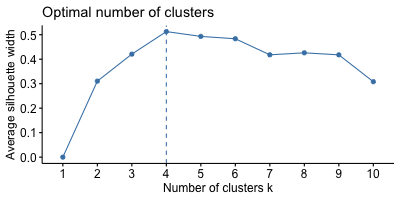
\includegraphics[width=5.56in]{images/silhouette} \hfill{}

\caption{ Silhoutte Indexes for Clusters \label{fig1}}\label{fig:unnamed-chunk-1}
\end{figure}

\begin{figure}[H]

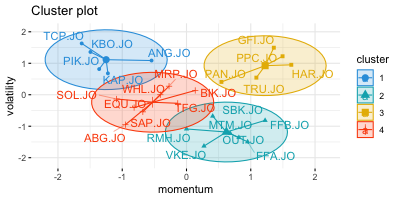
\includegraphics[width=5.56in]{images/clusters_image} \hfill{}

\caption{ Clusters Results from Highest Silhoutte \label{fig2}}\label{fig:unnamed-chunk-2}
\end{figure}

\hypertarget{portfolio-backtest}{%
\subsection{\texorpdfstring{Portfolio Backtest
\label{back}}{Portfolio Backtest }}\label{portfolio-backtest}}

The out-of-sample performance of cluster portfolios is compared to the
benchmark, the JSE All Share Index. To manage risk exposure to a single
asset or industry, we use a cap on each asset's allocation. Thus use a
single company methodology similar to Standard \& Poor Capping
Methodology \footnote{see S\&P (\protect\hyperlink{ref-sp}{2023}) for a
  breakdown of the process used to cap an index}. In a single company
capping methodology, no company in an index (cluster in our case) is
allowed to breach a certain pre-determined weight as of each rebalancing
period \footnote{The maximum set for each stock in each cluster is its
  equal weight for that cluster i.e if there were 10 stock in cluster 1,
  the maximum weight would be 10\%}. Theoretically, this should preserve
the within cluster diversification benefits and allow the portfolio
value to either increase or decrease depending on stock performance
during the quarter. We rebalance the portfolios once every three months,
similar to the frequency of rebalancing conducted by the JSE on the
JSE/FTSE indices, that is, re balance on the last daty of March, June,
September and December.

\hypertarget{results}{%
\section{\texorpdfstring{Results
\label{Results}}{Results }}\label{results}}

This section will present and analyze the clustering results of the
K-means algorithms. We will discuss constituent and cluster
charcateristics, hence show how we can uncover latent relationship
within stocks that based on factors that otherwise would be challenging.

\hypertarget{constiutent-description-in-clusters}{%
\subsection{Constiutent Description in
Clusters}\label{constiutent-description-in-clusters}}

In table \ref{tab1}, our ranking criterion and filtering lead to the
inclusion of three sectors: Basic Materials, Consumer Services, and
Financials. The ranking criterion assigns the highest score to stocks
that perform the best based on the specified factors. For instance, a
score close to 1 for the Price Momentum Rank indicates that a stock has
exhibited the strongest price movement over the past 12 months, while a
lower score suggests weaker performance. Similarly, for the Volatility
Rank, a score close to 1 signifies a stock with lower volatility, and a
lower score indicates higher volatility.

Examining Table \ref{tab1}, we observe that most stocks in the Financial
sector rank high in return volatility, Consumer Services stocks rank
low, and Basic Materials stocks rank even lower. Price Momentum ranks
Basic Materials stocks across the spectrum of Price Momnetum Rank, this
is similar for Financials and Consumer Services. Consequently, from the
ranking, there is no clear grouping by sector in terms of both price and
volatility.

Moving on to Table \ref{tab2}, where we apply K-means clustering and
determine the appropriate number of clusters to be K = 4, as suggested
by Figure \ref{fig1}. Notably, Cluster 2 predominantly comprises stocks
from the Financial sector, while Cluster 1, Cluster 3, and Cluster 4
exhibit a mix of representation from all sectors except Financials.
Additional details, including plots of rolling 12-month returns and
rolling 12-month standard deviation, can be found in Appendix \ref{app2}
\footnote{These plots illustrate similar movement in returns and
  volatility, providing insights into stock behavior over a one-year
  rolling period.It is important to note that these findings do not make
  a definitive case for a direct relationship among the securities but
  rather highlight the observed behavior over a specified time frame.}.

\hypertarget{results-from-rolling-backtest}{%
\subsection{Results from Rolling
Backtest}\label{results-from-rolling-backtest}}

Appendix \ref{app2} from \ref{tab3} to \ref{tab15} give a detailed
results of our rolling backtest. We aim to evaluate the performance of
these clusters over varying investment horizons, specifically focusing
on relative risk and return perspectives in comparison to the JSE All
Share Index. We add a modification to the methodology discussed in
\ref{back} designing a weight column constructed from relative volume
weighting. This approach ensures a thorough consideration of liquidity,
emphasizing the most liquid stocks within each cluster and have weights
to calulate execute our capping function.

Upon analyzing the final results, a noteworthy trend emerges --- the
clusters consistently demonstrate positive excess returns relative to
the benchmark. When holding the same clusters across investment horizons
ranging from 1 to 10 years, it becomes apparent that excess returns are
maximized in the shorter time frames. Specifically, over the short-term
(1 year from table \ref{tab4}), clusters generate superior excess
returns ranging from 30\% to 57\%, followed by 8.2\% to 10.8\% in the
medium term (5 years from table \ref{tab9}, and 4.8\% to 5.6\% over the
ultra-long term (10 years from table \ref{tab15}).

We notice consistency once we study the tracking error. Over the short
term, tracking errors range from 1.8\% to 7.9\%, followed by 10.2\% to
10.9\% in the medium term, and 9.9\% to 11.6\% in the long term. This
highlights the varying degrees of risk associated with the clusters
across different investment horizons. However, this tracking error
largely remains in tight ranges through the investment horizons.

Examining risk-adjusted metrics, we observe that clusters achieve a high
Sharpe Ratio (SR) of 2.3 in the short term. As the investment horizon
extends, the SR remains generally low but positive, suggesting that,
while the clusters may exhibit lower risk-adjusted returns over longer
periods, they continue to outperform in terms of risk efficiency in the
shorter term.

Lastly, Cluster 1 displays the least drawdowns and exhibits quick
recovery to previous from its maximum drawdown, particularly in very
short investment horizons. On the other hand, Cluster 3 consistently
experiences a more moderate level of drawdowns and recovery rates.
Notably, Clusters 1, 2, and 4 undergo a doubling of drawdowns from year
6 to year 7. However, over the long term, all clusters experience a
comparable level of drawdowns, with Cluster 4 showcasing the most
protracted recovery period from its down levels.

\hypertarget{conclusion}{%
\section{\texorpdfstring{Conclusion
\label{con}}{Conclusion }}\label{conclusion}}

Our objective was to develop a methodology utilizing factors with
theoretical foundations to unveil latent relationships among stocks
and/or sectors through the application of the K-means algorithm.
Additionally, we delved into return and risk metrics from a
retrospective standpoint, constructing a rolling backtest to assess the
robustness of the clustering results.

The obtained results indicate that cluster portfolios not only provide
positive excess returns but also demonstrate consistency in risk
relative to the benchmark. Over short periods, these portfolios generate
above-average risk-adjusted returns, albeit with the exception of the
lone high value observed in Cluster 1 over a one-year investment holding
period. A nuanced examination of the formed clusters reveals that a
single industry can make up an entire cluster, while a mix of industries
can compose another. This finding could be interpreted in various ways;
on one hand, it may suggest robust intra-sector relationships, allowing
for improved risk modeling. On the other hand, diverse clusters could
imply greater opportunities for sectoral rotation, depending on investor
capital expectations.

In conclusion, to enhance the comprehensiveness of this study, the
inclusion of additional factors, particularly fundamental ones, in our
K-means clustering framework could be considered. Furthermore, testing
various partition algorithms for their ability to form clusters with
high orthogonal risk drivers would contribute to a more thorough
analysis.

\newpage

\hypertarget{references}{%
\section{References}\label{references}}

\hypertarget{refs}{}
\begin{CSLReferences}{1}{0}
\leavevmode\vadjust pre{\hypertarget{ref-asness2011momentum}{}}%
Asness, C. 2011. Momentum in japan: The exception that proves the rule.
\emph{The Journal of Portfolio Management}. 37(4):67--75.

\leavevmode\vadjust pre{\hypertarget{ref-bin2020k}{}}%
Bin, S. 2020. K-means stock clustering analysis based on historical
price movements and financial ratios.

\leavevmode\vadjust pre{\hypertarget{ref-jegadeesh1993returns}{}}%
Jegadeesh, N. \& Titman, S. 1993. Returns to buying winners and selling
losers: Implications for stock market efficiency. \emph{The Journal of
finance}. 48(1):65--91.

\leavevmode\vadjust pre{\hypertarget{ref-kassambara2017practical}{}}%
Kassambara, A. 2017. \emph{Practical guide to cluster analysis in r:
Unsupervised machine learning}. Vol. 1. Sthda.

\leavevmode\vadjust pre{\hypertarget{ref-marvin2015creating}{}}%
Marvin, K. 2015. Creating diversified portfolios using cluster analysis.
\emph{Princeton University}.

\leavevmode\vadjust pre{\hypertarget{ref-rousseeuw1987silhouettes}{}}%
Rousseeuw, P.J. 1987. Silhouettes: A graphical aid to the interpretation
and validation of cluster analysis. \emph{Journal of computational and
applied mathematics}. 20:53--65.

\leavevmode\vadjust pre{\hypertarget{ref-sp}{}}%
S\&P. 2023. \emph{Index mathematics methodology}.

\leavevmode\vadjust pre{\hypertarget{ref-xu2010clustering}{}}%
Xu, R., Xu, J. \& Wunsch, D.C. 2010. Clustering with differential
evolution particle swarm optimization. In IEEE \emph{IEEE congress on
evolutionary computation}. 1--8.

\end{CSLReferences}

\newpage

\hypertarget{appendix}{%
\section{Appendix}\label{appendix}}

\hypertarget{appendix-a}{%
\subsection{\texorpdfstring{Appendix
A\label{app1}}{Appendix A}}\label{appendix-a}}

\begin{longtable}{rlrrl}
  \hline
 & Ticker & Price Momentum Rank & Volatility  Rank & Sector \\ 
  \hline
1 & ANG & 11.76 & 100.00 & Basic Materials \\ 
  2 & GFI & 82.35 & 94.12 & Basic Materials \\ 
  3 & PAN & 5.88 & 52.94 & Basic Materials \\ 
  4 & SAP & 52.94 & 64.71 & Basic Materials \\ 
  5 & MRP & 100.00 & 17.65 & Consumer Services \\ 
  6 & PIK & 35.29 & 70.59 & Consumer Services \\ 
  7 & TFG & 94.12 & 88.24 & Consumer Services \\ 
  8 & TRU & 23.53 & 82.35 & Consumer Services \\ 
  9 & WHL & 70.59 & 76.47 & Consumer Services \\ 
  10 & ABG & 76.47 & 47.06 & Financials \\ 
  11 & EQU & 17.65 & 23.53 & Financials \\ 
  12 & FFA & 29.41 & 5.88 & Financials \\ 
  13 & MTM & 47.06 & 41.18 & Financials \\ 
  14 & OUT & 88.24 & 35.29 & Financials \\ 
  15 & SBK & 41.18 & 29.41 & Financials \\ 
  16 & VKE & 58.82 & 11.76 & Financials \\ 
  17 & KAP & 64.71 & 58.82 & Industrials \\ 
   \hline
\hline
\caption{Stock Ranking By Factors \label{tab1}} 
\end{longtable}

\begin{table}[H]
\centering
\begin{tabular}{rlrl}
  \hline
 & Ticker & Cluster & Sector \\ 
  \hline
1 & ABG.JO &   1 & Financials \\ 
  2 & MRP.JO &   1 & Consumer Services \\ 
  3 & OUT.JO &   1 & Financials \\ 
  4 & EQU.JO &   2 & Financials \\ 
  5 & FFA.JO &   2 & Financials \\ 
  6 & MTM.JO &   2 & Financials \\ 
  7 & SBK.JO &   2 & Financials \\ 
  8 & VKE.JO &   2 & Financials \\ 
  9 & ANG.JO &   3 & Basic Materials \\ 
  10 & PAN.JO &   3 & Basic Materials \\ 
  11 & PIK.JO &   3 & Consumer Services \\ 
  12 & TRU.JO &   3 & Consumer Services \\ 
  13 & GFI.JO &   4 & Basic Materials \\ 
  14 & KAP.JO &   4 & Industrials \\ 
  15 & SAP.JO &   4 & Basic Materials \\ 
  16 & TFG.JO &   4 & Consumer Services \\ 
  17 & WHL.JO &   4 & Consumer Services \\ 
   \hline
\end{tabular}
\caption{Stock Classification by Sector and Cluster \label{tab2}} 
\end{table}

\newpage

\newpage

\hypertarget{appendix-b}{%
\section{\texorpdfstring{Appendix B
\label{app2}}{Appendix B }}\label{appendix-b}}

\begin{figure}[H]

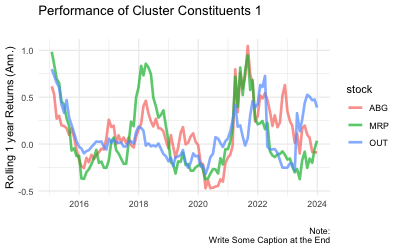
\includegraphics[width=5.56in]{images/returnplots_1} \hfill{}

\caption{ Clusters Results from Highest Silhoutte \label{fig2}}\label{fig:unnamed-chunk-5-1}
\end{figure}
\begin{figure}[H]

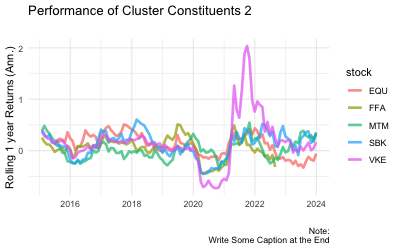
\includegraphics[width=5.56in]{images/returnplots_2} \hfill{}

\caption{ Clusters Results from Highest Silhoutte \label{fig2}}\label{fig:unnamed-chunk-5-2}
\end{figure}
\begin{figure}[H]

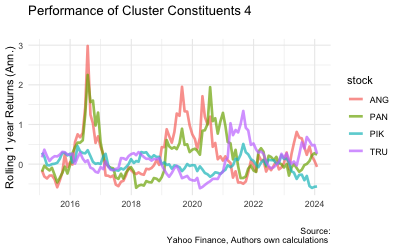
\includegraphics[width=5.56in]{images/returnplots_4} \hfill{}

\caption{ Clusters Results from Highest Silhoutte \label{fig2}}\label{fig:unnamed-chunk-5-3}
\end{figure}
\begin{figure}[H]

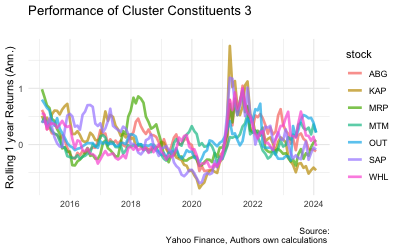
\includegraphics[width=5.56in]{images/returnplots_3} \hfill{}

\caption{ Clusters Results from Highest Silhoutte \label{fig2}}\label{fig:unnamed-chunk-5-4}
\end{figure}

\begin{figure}[H]

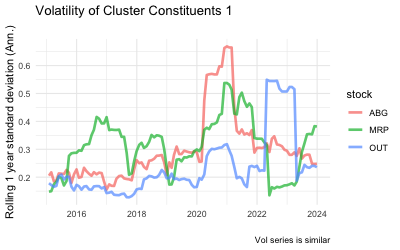
\includegraphics[width=5.56in]{images/volplots_1} \hfill{}

\caption{ Clusters Results from Highest Silhoutte \label{fig2}}\label{fig:unnamed-chunk-6-1}
\end{figure}
\begin{figure}[H]

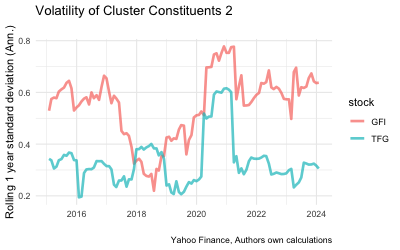
\includegraphics[width=5.56in]{images/volplots_2} \hfill{}

\caption{ Clusters Results from Highest Silhoutte \label{fig2}}\label{fig:unnamed-chunk-6-2}
\end{figure}
\begin{figure}[H]

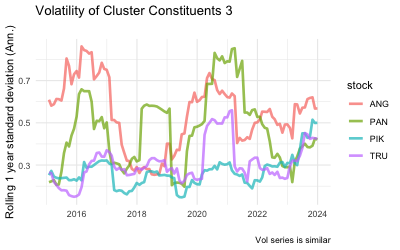
\includegraphics[width=5.56in]{images/volplots_3} \hfill{}

\caption{ Clusters Results from Highest Silhoutte \label{fig2}}\label{fig:unnamed-chunk-6-3}
\end{figure}
\begin{figure}[H]

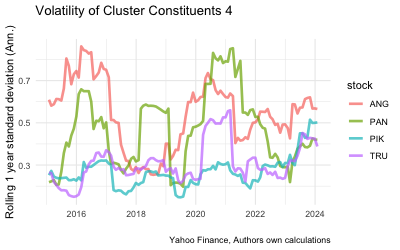
\includegraphics[width=5.56in]{images/volplots_4} \hfill{}

\caption{ Clusters Results from Highest Silhoutte \label{fig2}}\label{fig:unnamed-chunk-6-4}
\end{figure}
\newpage

\hypertarget{look-back}{%
\subsection{Look Back}\label{look-back}}

\begin{longtable}{rllrrrr}
\caption{LookBack Performance \label{tab3}} \\ 
  \hline
 & Period & Info & X1 & X3 & X4 & X2 \\ 
  \hline
1 & Last 12 Months & Adj. Sharpe Ratio & 0.17 & 0.18 & 0.23 & 0.12 \\ 
  2 & Last 12 Months & Avg DD & 0.13 & 0.15 & 0.17 & 0.12 \\ 
  3 & Last 12 Months & Beta & 1.11 & 0.69 & 0.97 & 1.20 \\ 
  4 & Last 12 Months & Beta Bear & 1.97 & 0.01 & 1.30 & 2.05 \\ 
  5 & Last 12 Months & Beta Bull & 1.05 & 1.43 & 0.52 & 1.41 \\ 
  6 & Last 12 Months & Returns Excess (Ann.) & 0.06 & 0.05 & 0.06 & 0.05 \\ 
  7 & Last 12 Months & Tracking Error & 0.20 & 0.19 & 0.20 & 0.17 \\ 
   \hline
\hline
\end{longtable}

\begin{longtable}{rllrrrr}
\caption{LookBack Performance \label{tab4}} \\ 
  \hline
 & Period & Info & X1 & X3 & X4 & X2 \\ 
  \hline
1 & Last 3 Months & Adj. Sharpe Ratio & 0.43 & 0.17 & 1.37 & 0.25 \\ 
  2 & Last 3 Months & Avg DD & 0.10 & 0.07 & 0.03 & 0.09 \\ 
  3 & Last 3 Months & Beta & 1.11 & 0.46 & 0.53 & 1.29 \\ 
  4 & Last 3 Months & Beta Bear & 1.19 & 0.55 & 1.20 & 1.87 \\ 
  5 & Last 3 Months & Beta Bull & 0.55 & -0.15 & -2.46 & -0.24 \\ 
  6 & Last 3 Months & Returns Excess (Ann.) & 0.13 & 0.09 & 0.21 & 0.11 \\ 
  7 & Last 3 Months & Tracking Error & 0.16 & 0.17 & 0.17 & 0.13 \\ 
   \hline
\hline
\end{longtable}

\begin{longtable}{rllrrrr}
\caption{LookBack Performance \label{tab5}} \\ 
  \hline
 & Period & Info & X1 & X3 & X4 & X2 \\ 
  \hline
1 & Last 6 Months & Adj. Sharpe Ratio & -0.06 & 0.55 & 0.23 & 0.07 \\ 
  2 & Last 6 Months & Avg DD & 0.35 & 0.06 & 0.10 & 0.17 \\ 
  3 & Last 6 Months & Beta & 1.16 & 0.57 & 1.06 & 1.19 \\ 
  4 & Last 6 Months & Beta Bear & 2.20 & 0.37 & 1.56 & 2.38 \\ 
  5 & Last 6 Months & Beta Bull & 1.09 & 1.35 & 0.77 & 0.70 \\ 
  6 & Last 6 Months & Returns Excess (Ann.) & 0.03 & 0.10 & 0.08 & 0.05 \\ 
  7 & Last 6 Months & Tracking Error & 0.20 & 0.17 & 0.20 & 0.18 \\ 
   \hline
\hline
\end{longtable}
\newpage

\hypertarget{rolling-backtest-results}{%
\subsection{Rolling Backtest Results}\label{rolling-backtest-results}}

\begin{table}[H]
\centering
\caption{Rolling Performance Performance \label{tab6}} 
\begin{tabular}{rllrrrr}
  \hline
 & Investment Horizon & Info & Cluster\_1 & Cluster\_3 & Cluster\_4 & Cluster\_2 \\ 
  \hline
1 & 1 Year & Ann Excess Return & 0.58 & 0.31 & 0.46 & 0.36 \\ 
  2 & 1 Year & Ann Tracking Error & 0.08 & 0.13 & 0.12 & 0.02 \\ 
  3 & 1 Year & Adj. Sharpe Ratio & 2.33 & -0.17 & 0.65 & 0.30 \\ 
  4 & 1 Year & DD Length & 2.00 & 3.00 & 3.00 & 3.00 \\ 
  5 & 1 Year & Max DD & 0.00 & 0.12 & 0.06 & 0.02 \\ 
   \hline
\end{tabular}
\end{table}

\begin{longtable}{rllrrrr}
\caption{Rolling Performance Performance \label{tab7}} \\ 
  \hline
 & Investment Horizon & Info & Cluster\_1 & Cluster\_3 & Cluster\_4 & Cluster\_2 \\ 
  \hline
1 & 2 Year & Ann Excess Return & 0.18 & 0.10 & 0.14 & 0.10 \\ 
  2 & 2 Year & Ann Tracking Error & 0.10 & 0.12 & 0.10 & 0.08 \\ 
  3 & 2 Year & Adj. Sharpe Ratio & 0.20 & -0.38 & -0.11 & -0.63 \\ 
  4 & 2 Year & DD Length & 3.00 & 7.00 & 7.00 & 4.00 \\ 
  5 & 2 Year & Max DD & 0.12 & 0.24 & 0.16 & 0.14 \\ 
   \hline
\hline
\end{longtable}

\begin{longtable}{rllrrrr}
\caption{Rolling Performance Performance \label{tab8}} \\ 
  \hline
 & Investment Horizon & Info & Cluster\_1 & Cluster\_3 & Cluster\_4 & Cluster\_2 \\ 
  \hline
1 & 3 Year & Ann Excess Return & 0.17 & 0.13 & 0.14 & 0.15 \\ 
  2 & 3 Year & Ann Tracking Error & 0.10 & 0.13 & 0.12 & 0.09 \\ 
  3 & 3 Year & Adj. Sharpe Ratio & 0.59 & 0.18 & 0.25 & 0.35 \\ 
  4 & 3 Year & DD Length & 4.00 & 6.00 & 11.00 & 4.00 \\ 
  5 & 3 Year & Max DD & 0.12 & 0.24 & 0.16 & 0.14 \\ 
   \hline
\hline
\end{longtable}

\begin{longtable}{rllrrrr}
\caption{Rolling Performance Performance \label{tab9}} \\ 
  \hline
 & Investment Horizon & Info & Cluster\_1 & Cluster\_3 & Cluster\_4 & Cluster\_2 \\ 
  \hline
1 & 4 Year & Ann Excess Return & 0.16 & 0.05 & 0.11 & 0.11 \\ 
  2 & 4 Year & Ann Tracking Error & 0.11 & 0.12 & 0.11 & 0.09 \\ 
  3 & 4 Year & Adj. Sharpe Ratio & 0.69 & -0.19 & 0.25 & 0.27 \\ 
  4 & 4 Year & DD Length & 4.00 & 8.00 & 15.00 & 5.00 \\ 
  5 & 4 Year & Max DD & 0.12 & 0.24 & 0.16 & 0.14 \\ 
   \hline
\hline
\end{longtable}

\begin{longtable}{rllrrrr}
\caption{Rolling Performance Performance \label{tab10}} \\ 
  \hline
 & Investment Horizon & Info & Cluster\_1 & Cluster\_3 & Cluster\_4 & Cluster\_2 \\ 
  \hline
1 & 5 Year & Ann Excess Return & 0.11 & 0.07 & 0.09 & 0.08 \\ 
  2 & 5 Year & Ann Tracking Error & 0.11 & 0.13 & 0.10 & 0.10 \\ 
  3 & 5 Year & Adj. Sharpe Ratio & 0.41 & 0.08 & 0.22 & 0.19 \\ 
  4 & 5 Year & DD Length & 4.00 & 10.00 & 19.00 & 4.00 \\ 
  5 & 5 Year & Max DD & 0.12 & 0.24 & 0.16 & 0.14 \\ 
   \hline
\hline
\end{longtable}

\begin{longtable}{rllrrrr}
\caption{Rolling Performance Performance \label{tab11}} \\ 
  \hline
 & Investment Horizon & Info & Cluster\_1 & Cluster\_3 & Cluster\_4 & Cluster\_2 \\ 
  \hline
1 & 6 Year & Ann Excess Return & 0.08 & 0.06 & 0.06 & 0.09 \\ 
  2 & 6 Year & Ann Tracking Error & 0.11 & 0.12 & 0.11 & 0.10 \\ 
  3 & 6 Year & Adj. Sharpe Ratio & 0.28 & 0.09 & 0.04 & 0.39 \\ 
  4 & 6 Year & DD Length & 6.00 & 12.00 & 23.00 & 5.00 \\ 
  5 & 6 Year & Max DD & 0.16 & 0.24 & 0.16 & 0.14 \\ 
   \hline
\hline
\end{longtable}

\begin{longtable}{rllrrrr}
\caption{Rolling Performance Performance \label{tab12}} \\ 
  \hline
 & Investment Horizon & Info & Cluster\_1 & Cluster\_3 & Cluster\_4 & Cluster\_2 \\ 
  \hline
1 & 7 Year & Ann Excess Return & 0.06 & 0.07 & 0.04 & 0.06 \\ 
  2 & 7 Year & Ann Tracking Error & 0.12 & 0.12 & 0.11 & 0.11 \\ 
  3 & 7 Year & Adj. Sharpe Ratio & 0.08 & 0.19 & -0.03 & 0.09 \\ 
  4 & 7 Year & DD Length & 6.00 & 13.00 & 27.00 & 5.00 \\ 
  5 & 7 Year & Max DD & 0.35 & 0.24 & 0.30 & 0.26 \\ 
   \hline
\hline
\end{longtable}

\begin{longtable}{rllrrrr}
\caption{Rolling Performance Performance \label{tab13}} \\ 
  \hline
 & Investment Horizon & Info & Cluster\_1 & Cluster\_3 & Cluster\_4 & Cluster\_2 \\ 
  \hline
1 & 8 Year & Ann Excess Return & 0.06 & 0.04 & 0.04 & 0.06 \\ 
  2 & 8 Year & Ann Tracking Error & 0.12 & 0.11 & 0.11 & 0.10 \\ 
  3 & 8 Year & Adj. Sharpe Ratio & 0.16 & 0.05 & 0.03 & 0.15 \\ 
  4 & 8 Year & DD Length & 8.00 & 10.00 & 31.00 & 6.00 \\ 
  5 & 8 Year & Max DD & 0.35 & 0.24 & 0.30 & 0.26 \\ 
   \hline
\hline
\end{longtable}

\begin{longtable}{rllrrrr}
\caption{Rolling Performance Performance \label{tab14}} \\ 
  \hline
 & Investment Horizon & Info & Cluster\_1 & Cluster\_3 & Cluster\_4 & Cluster\_2 \\ 
  \hline
1 & 9 Year & Ann Excess Return & 0.05 & 0.04 & 0.05 & 0.04 \\ 
  2 & 9 Year & Ann Tracking Error & 0.12 & 0.11 & 0.11 & 0.10 \\ 
  3 & 9 Year & Adj. Sharpe Ratio & 0.12 & 0.05 & 0.10 & 0.04 \\ 
  4 & 9 Year & DD Length & 8.00 & 12.00 & 35.00 & 5.00 \\ 
  5 & 9 Year & Max DD & 0.35 & 0.24 & 0.30 & 0.26 \\ 
   \hline
\hline
\end{longtable}

\begin{longtable}{rllrrrr}
\caption{Rolling Performance Performance \label{tab15}} \\ 
  \hline
 & Investment Horizon & Info & Cluster\_1 & Cluster\_3 & Cluster\_4 & Cluster\_2 \\ 
  \hline
1 & 10 Year & Ann Excess Return & 0.06 & 0.05 & 0.06 & 0.05 \\ 
  2 & 10 Year & Ann Tracking Error & 0.12 & 0.11 & 0.11 & 0.10 \\ 
  3 & 10 Year & Adj. Sharpe Ratio & 0.17 & 0.18 & 0.23 & 0.12 \\ 
  4 & 10 Year & DD Length & 10.00 & 10.00 & 18.00 & 6.00 \\ 
  5 & 10 Year & Max DD & 0.35 & 0.24 & 0.30 & 0.26 \\ 
   \hline
\hline
\end{longtable}

\bibliography{Tex/ref}





\end{document}
